Aside from dropout in the final layer, we employ no regularization methods on 
our models. \citet{lstm_third_paper} 
argue that there is evidence that adding so-called "physical constraints" to 
models used on CAMELS could be helpful. This is argued because the LSTM models 
underperform compared to SAC-SMA on some basins. Here the paper compares SAC-SMA 
to an LSTM trained on all basins, training and validation split time series-wise 
and not basin-wise. SAC-SMA is a conceptual model and is therefore not usually seen 
as a purely "physical" model, but it is based more on physical arguments than a 
generalized machine learning method, as it is "conceptually" based on the real world.
Still, both SAC-SMA and the LSTM are essentially 
parameter based models, without clear physical interpretations of most parameters. 
Because of this, we are unsure whether the argument that this is evidence for physical 
constraints is sufficient. More research is needed on the topic. Regularization in 
the form of physical constraints may yield several benefits, some of which could be
\citep{hybrid_paper}:
\begin{itemize}
\item Interpretability: Physical constraints could improve the physical interpretability 
of the LSTM.
\item Improved generalization: The goal of most machine learning regularization is 
to improve performance by increasing bias and decreasing variance (see Figure 
\ref{Bias Variance rainfall}). Increasing bias using physical laws would fit well 
into the narrative of \citet{BiasVarianceVIC} and \citet{VICbench}, although from 
the opposite angle. These papers argue that process-driven models are often too 
statistically constrained, due to them being driven almost entirely by interpretable 
physical processes. \citet{VICbench} showed that VIC performs at a higher level 
when tuning more parameters than usual, as these parameters are often pre-set based 
on physical a-priori knowledge. This is analogous to the bias-variance trade-off 
in machine learning. An LSTM is much less constrained and therefore performs better, 
agreeing with the results of the aforementioned papers. Making LSTM models 
slightly more constrained (as worded by \citet{BiasVarianceVIC}) could then make 
them generalize successfully to more basins while still being powerful enough to 
learn necessary relationships between input variables.
\end{itemize}
In the spirit of \citet{hybrid_paper}'s argument for increasing the physical consistency 
of models, we propose a simple semi-physical constraint:
\begin{equation}
\bm{\hat{y}} = \text{LSTM}(\bm{x}),
\end{equation}
where $\bm{\hat{y}}$ now consists of three outputs: $\bm{y}_\text{discharge}$, 
$\bm{y}_\text{frost}$ and $\bm{y}_\text{radiation}$. These represent runoff, 
frost/snow and radiated water respectively. Only $\bm{y}_\text{discharge}$ would 
be treated as the actual input when calculating the original cost function 
(\ref{NSE loss}). We then introduce a long term frost storage variable $\bm{W}^t_\text{frost}$.
For each time step this storage variable is updated by 
\begin{equation}
    \bm{W}_\text{frost}^{t+1} = \bm{W}_\text{frost}^t + \bm{y}_\text{frost},
\end{equation}
where $t$ is the current time step.
When calculating the loss function, we now add a new term to (\ref{NSE loss}):
\begin{equation}
    L = \text{NSE}^* + \gamma \left|(\bm{y_\text{discharge}} - \bm{x}_\text{precipitation} 
    - \bm{y}_\text{radiation} - (\bm{y}_\text{frost} - \bm{W}_\text{frost}))\right|
    \label{physical constraint}.
\end{equation}
Here $\gamma$ is a hyperparameter that needs to be tuned. Our reasoning 
behind (\ref{physical constraint}) is that this cost function penalizes models for 
making predictions where there is more runoff than available precipitation, 
snow and frost. Our hypothesis is that this penalty should lead to less complex 
models that are less likely to predict unphysical behaviors, leading to 
fewer NSE scores below zero. It could also improve interpretability of the model's 
output. Whether this or a similar constraint behaves as intended remains to be seen.

\begin{figure}
\centering


%\tikzset{every picture/.style={line width=0.75pt}} %set default line width to 0.75pt        

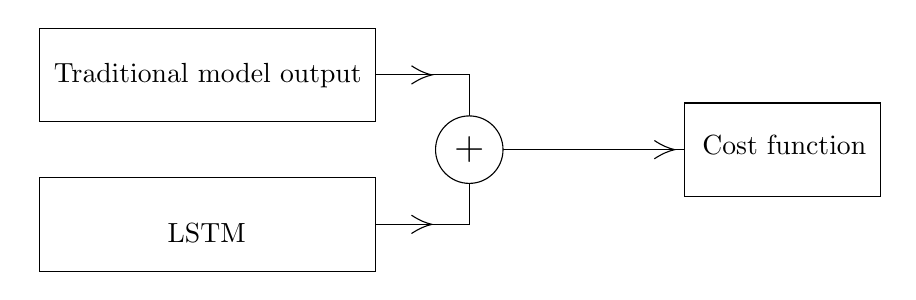
\begin{tikzpicture}[x=0.75pt,y=0.75pt,yscale=-0.9,xscale=0.9]
%uncomment if require: \path (0,300); %set diagram left start at 0, and has height of 300

%Shape: Right Angle [id:dp6736520719365272] 
\draw   (320,50) -- (370,50) -- (370,90) ;
%Shape: Right Angle [id:dp1824696211077277] 
\draw   (370,90) -- (370,130) -- (320,130) ;
%Straight Lines [id:da5169071611896188] 
\draw    (370,90) -- (485,90) ;
\draw [shift={(480,90)}, rotate = 180] [color={rgb, 255:red, 0; green, 0; blue, 0 }  ]   (10.93,-4.9) .. controls (6.95,-2.3) and (3.31,-0.67) .. (0,0) .. controls (3.31,0.67) and (6.95,2.3) .. (10.93,4.9)   ;
\draw [shift={(350,50)}, rotate = 180] [color={rgb, 255:red, 0; green, 0; blue, 0 }  ]   (10.93,-4.9) .. controls (6.95,-2.3) and (3.31,-0.67) .. (0,0) .. controls (3.31,0.67) and (6.95,2.3) .. (10.93,4.9)   ;
\draw [shift={(350,130)}, rotate = 180] [color={rgb, 255:red, 0; green, 0; blue, 0 }  ]   (10.93,-4.9) .. controls (6.95,-2.3) and (3.31,-0.67) .. (0,0) .. controls (3.31,0.67) and (6.95,2.3) .. (10.93,4.9)   ;
%\draw   (336,44.92) .. controls (340.03,47.37) and (344.07,48.84) .. (348.1,49.33) .. controls (344.07,49.82) and (340.03,51.3) .. (336,53.75) ;
%\draw   (338.5,130.08) .. controls (342.53,132.54) and (346.57,134.01) .. (350.6,134.5) .. controls (346.57,134.99) and (342.53,136.46) .. (338.5,138.92) ;

% Text Node
\draw    (140,25) -- (320,25) -- (320,75) -- (140,75) -- cycle  ;
\draw (230,50.2) node   [align=left] {\begin{minipage}[lt]{122.67200000000003pt}\setlength\topsep{0pt}
\begin{center}
Traditional model output
\end{center}

\end{minipage}};
% Text Node
\draw    (140,105) -- (320,105) -- (320,155) -- (140,155) -- cycle  ;
\draw (229.4,134.6) node   [align=left] {\begin{minipage}[lt]{122.67200000000003pt}\setlength\topsep{0pt}
\begin{center}
LSTM
\end{center}

\end{minipage}};
% Text Node
\draw  [fill={rgb, 255:red, 255; green, 255; blue, 255 }  ,fill opacity=1 ]  (370, 90) circle [x radius= 18.06, y radius= 18.06]   ;
\draw (370,90) node   [align=left] {\begin{minipage}[lt]{16.864pt}\setlength\topsep{0pt}
\begin{center}
{\Large +}
\end{center}

\end{minipage}};
% Text Node
\draw    (485,65) -- (590,65) -- (590,115) -- (485,115) -- cycle  ;
\draw (538.6,87.4) node   [align=left] {\begin{minipage}[lt]{68pt}\setlength\topsep{0pt}
\begin{center}
Cost function
\end{center}

\end{minipage}};


\end{tikzpicture}

.tex}
    \caption[Potential simple hybrid model.]{Sketch of how a simple hybrid model could be implemented. The traditional model and the LSTM model are completely separate, making it unnecessary to calculate gradients for the traditional model. The idea here would be for the LSTM model to learn the phenomena lacking in traditional models.}
\label{figure simple hybrid}
\end{figure}
Sticking to the topic of increased generalizability and interpretability, we 
believe it to be of interest to implement a hybrid model, i. e. a machine learning 
model implemented alongside or as part of a 
traditional model. The machine learning model either replaces parts of or supplements 
the predictions of a traditional model. A very simple implementation of this is shown 
in Figure \ref{figure simple hybrid}. This model would take the same inputs as 
the models trained in this thesis, but the cost function would be calculated on 
the sum of the output of the traditional model and the machine learning model. 
This means that the machine learning model learns to correct 
the errors of a given traditional model instead of doing actual prediction.

This thesis and earlier research done by \citet{lstm_first_paper,lstm_second_paper,lstm_third_paper} 
are all limited to simple LSTM models. LSTM models are, due to their recurrent nature, 
notoriously slow. Graphics cards and similar highly parallel computational devices 
are not optimized for recurrent calculation. A relatively 
simple way to surpass this could be to implement a one-dimensional 
Convolutional Neural Network (CNN) layer as the first layer of our model. This 
layer could then be used to reduce the time resolution of the data, still retaining 
information. The usage of CNNs for time series prediction is becoming increasingly
widespread \citep{CNN-timeseries}. We still argue that LSTM models fit the type of
physical system modelled in this thesis very well and is logically consistent 
with the way rainfall-runoff 
models are typically structured, but using a CNN layer to improve performance 
should not detract from this.
